\documentclass[11pt]{article}
\usepackage[a4paper,margin=2.3cm]{geometry}
\usepackage{amsmath,amssymb,booktabs,graphicx,subcaption,hyperref,xcolor}
\usepackage[numbers,sort]{natbib}
\hypersetup{colorlinks=true,linkcolor=blue!50!black,citecolor=blue!50!black,urlcolor=blue!50!black}
\newcommand{\Sv}{S}

\title{Learning Segment Costs Through a Differentiable Segment-Viterbi\\for True Vertical Thickness Prediction in Horizontal Wells}
\author{Tabish Shah Mohsin\\{\small Department of Computer Engineering, ZHCET, Aligarh Muslim University}}
\date{Technical report, November 2026}

\begin{document}
\maketitle

\begin{abstract}
We predict true vertical thickness (TVT) along the lateral of a horizontal well from its gamma-ray (GR) log, a vertical typewell GR log and the well trajectory. The task comes from the Kaggle ROGII Wellbore Geology Prediction competition. We cast the stratigraphic path as a piecewise-linear curve on a fixed lattice of anchor depths. A small neural network scores each candidate straight segment, and the network is trained \emph{through} the dynamic program. A soft (log-sum-exp) Viterbi forward--backward pass turns segment costs into an expected path, and the mean squared TVT error of that path is back-propagated to the cost network. The released cost network has only \textbf{1{,}271 parameters}.

On a 155-well validation fold it reduces the hard-path RMSE from 13.98\,ft (hand-crafted GR misfit cost) to 5.95--6.58\,ft (two independent training runs). For comparison, our own ${\sim}50$M-parameter whole-lateral CNN reaches 5.64\,ft on the same fold. On the competition's hidden test set the model scores 7.724 private / 9.551 public RMSE.

An error analysis shows that the lattice is not the limitation: the best path the grid allows is within ${\approx}0.25$\,ft of the truth. Error concentrates in a few wells where the decoder commits to a wrong branch: 20 of 155 wells carry 70\% of the squared error. In most of these wells a near-tied alternative path is already among the model's top candidates. The best of the top-4 distinct paths would score 4.10\,ft, which points to whole-lateral re-ranking as the next step.
\end{abstract}

\section{Introduction}
Geosteering keeps a horizontal well inside a target formation by continuously estimating where the bit sits stratigraphically. A standard quantitative target is the true vertical thickness (TVT): the vertical stratigraphic depth of each lateral sample measured in the coordinate system of a vertical reference ``typewell''. While drilling, the lateral GR log is matched against the typewell GR log, and the interpreter adjusts the assumed dip of the layers until the two logs agree.

The ROGII competition \citep{rogii2026} provides 773 training laterals with the known TVT. For each well, TVT is given up to a cut-off point and must be predicted for the remainder of the lateral; the score is the RMSE in feet. The strongest public solutions are dense image models: 2D alignment-probability networks over (lateral position $\times$ candidate depth) with neighbour-well channels, and an anchor-CNN whose outputs are decoded by dynamic programming. In these, the network is trained with a classification or regression loss and the structural decoding is a separate, non-learned post-process.

\paragraph{Contribution.} We study the opposite design: a very small learned cost inside an explicit structural model, trained end-to-end through the decoder.
\begin{itemize}
\item We formulate TVT prediction as a shortest path on a segment lattice in a detrended structural coordinate (Sec.~\ref{sec:lattice}). The prediction is piecewise linear in that coordinate, with a hard dip limit.
\item We learn the segment cost with a 1{,}271-parameter convolutional network and train it through a soft Viterbi forward--backward recursion with an MSE loss on TVT (Sec.~\ref{sec:soft}). This follows differentiable dynamic programming \citep{mensch2018diffdp,cuturi2017softdtw}, applied here to a geological path model.
\item We report ablations, a held-out test score and a detailed error analysis (Sec.~\ref{sec:results}). The analysis locates the residual error in decoder branch choice rather than in lattice resolution or local matching.
\end{itemize}

\section{Data and task}
Each well provides a lateral table sampled every 1\,ft of measured depth (MD), with columns MD, $X$, $Y$, $Z$ (true vertical depth, negative down), GR and \texttt{TVT\_input}. \texttt{TVT\_input} holds the known TVT up to row $K$ and is missing afterwards. Each well also provides a typewell table of (TVT, GR) pairs. The target is TVT for rows $K,\dots,n-1$.

We use a 5-fold split of the 773 training wells: sorted well names, random permutation with seed 42, fold = index mod 5. All validation numbers in this report are for \textbf{fold 0} (155 wells; the model is trained on the other 618). They are pooled RMSE over all predicted rows of all validation wells, so long wells weigh more. The hidden-test numbers are from Kaggle's re-run of our inference notebook.

\section{Method}
\subsection{Structural coordinate and lattice}\label{sec:lattice}
For a flat layer, TVT$+Z$ is constant along the lateral. We fit a straight line to the lateral's $Z$ against MD, $Z_{\mathrm{lin}}(s)=m_zs+c_z$, and work in the detrended coordinate
\begin{equation}
\Sv(s)\;=\;\mathrm{TVT}(s)-z_{\det}(s)-\mathrm{TVT}_0,\qquad z_{\det}(s)=Z_{\mathrm{lin}}(s)-Z(s),
\end{equation}
where $\mathrm{TVT}_0$ is the last known TVT. $\Sv\equiv$ const describes layers parallel to the well's mean trajectory, which we call the \emph{straight baseline}. In this coordinate the true paths are close to piecewise linear: they have long straight runs and only a few kinks per well (Fig.~\ref{fig:sspace}).

The prediction region is cut into chunks of $L=80$ rows (80\,ft). At boundary $i$ (distance $r_i$ rows from the cut-off) we place anchors on a 1\,ft grid,
\begin{equation}
\mathcal{A}_i=\{\Sv_0+k:\;|k|\le\min(0.05\,r_i,\,100)\},
\end{equation}
which gives 9 anchors at the first boundary and 201 after ${\approx}2{,}000$\,ft. A candidate segment joins $a\in\mathcal{A}_i$ to $b\in\mathcal{A}_{i+1}$ with $|b-a|/L\le 0.05$, i.e.\ at most a 3$^\circ$ apparent dip relative to the baseline. That is $\le 9$ successors per anchor and about 1{,}300 segments per chunk on average.

The prediction is the straight-line interpolation of the chosen anchors, mapped back to TVT. Using the true $\Sv$ at the boundaries (the \emph{grid best fit}) reproduces the truth to ${\approx}0.25$\,ft RMSE on fold-0 wells, so the lattice itself costs almost nothing.

\subsection{Segment features}
For segment $(a,b)$ with slope $m=(b-a)/L$ we extend its line one chunk backwards and one chunk forwards and sample 48 equally spaced points (16 per chunk). At each point we form five channels:
\begin{itemize}
\item $g$: the lateral GR, low-pass filtered, box-averaged and standardised by the typewell GR mean and standard deviation within $\pm200$\,ft of $\mathrm{TVT}_0$;
\item $t$: the typewell GR read at $\mathrm{TVT}=\Sv_{\text{line}}+z_{\det}+\mathrm{TVT}_0$, i.e.\ what the typewell predicts if the line is correct;
\item $g-t$;
\item $(\Sv_{\text{line}}-\Sv_{\text{nb}})/10$, the offset from a neighbour-field prediction (below);
\item a mask marking the current chunk.
\end{itemize}

Six scalars complete the input:
\begin{itemize}
\item $20m$;
\item $20(m-m_{\text{nb}})$, the slope relative to the neighbour field's slope over the chunk;
\item the chunk start position divided by 4000;
\item the mean offset from the neighbour field divided by 20;
\item the \emph{hand cost} $h=\overline{(g-t)^2}$ over the current chunk;
\item $\overline{(g-t)^2}$ over the whole window.
\end{itemize}

\paragraph{Neighbour field.} We estimate a map-view structural gradient of TVT$+Z$ from along-track dip observations of nearby labelled wells, plus the query well's own known build section. The fit is a Gaussian-weighted least squares with ridge shrinkage to the regional gradient and one Tukey reweighting pass. Integrating this gradient along the query trajectory gives $\Sv_{\text{nb}}$. For training wells the support set excludes the validation fold; at test time all 773 wells are used.

\subsection{Cost network}
The cost of a segment is
\begin{equation}
c_\theta(a,b)=\frac{L_i}{80}\Big(w\,h+\mathrm{MLP}\big([\mathrm{mean}(\phi),\,\max(\phi),\,\text{scalars}]\big)\Big),\qquad \phi=\mathrm{CNN}(\text{5-channel sequence}).
\end{equation}
The CNN is Conv1d(5$\to$12, kernel 5)--ReLU--MaxPool(2)--Conv1d(12$\to$12, kernel 3)--ReLU. The MLP is Linear(30$\to$16)--ReLU--Linear(16$\to$1), with its last layer initialised to zero, so training starts exactly at the hand cost ($w=1$). Table~\ref{tab:params} lists the parameters: 1{,}271 in total, including the hand-cost weight $w$ and the log-temperature.

\begin{table}[h]\centering\small
\begin{tabular}{lr}
\toprule
Layer & Parameters\\\midrule
Conv1d 5$\to$12, $k{=}5$ & 312\\
Conv1d 12$\to$12, $k{=}3$ & 444\\
Linear 30$\to$16 & 496\\
Linear 16$\to$1 & 17\\
hand-cost weight $w$, log-temperature $\log T$ & 2\\\midrule
\textbf{Total} & \textbf{1{,}271}\\
\bottomrule
\end{tabular}
\caption{Size of the released cost network. The stored weights file is 9.2\,kB.}\label{tab:params}
\end{table}

\subsection{Soft Viterbi and training loss}\label{sec:soft}
Let $C_i\in\mathbb{R}^{|\mathcal{A}_i|\times|\mathcal{A}_{i+1}|}$ hold the segment costs of chunk $i$, with $+\infty$ (numerically $10^4$) for disallowed transitions. The hard decoder is the Viterbi recursion \citep{viterbi1967,forney1973}. For training we replace $\min$ by the smooth minimum $\min_T(x)=-T\log\sum_j e^{-x_j/T}$:
\begin{align}
\alpha_{i+1}(b)&=\min\nolimits_T\big\{\alpha_i(a)+C_i(a,b)\big\}_a, &
\beta_i(a)&=\min\nolimits_T\big\{C_i(a,b)+\beta_{i+1}(b)\big\}_b,\\
p_i(a)&=\operatorname{softmax}_a\!\big(-(\alpha_i(a)+\beta_i(a))/T\big), &
\hat\Sv_i&=\textstyle\sum_a p_i(a)\,a .
\end{align}
The expected anchors $\hat\Sv_i$ are linearly interpolated to every row and mapped to TVT. The loss is the mean squared TVT error over the well, back-propagated through $\alpha,\beta$ into $c_\theta$; $T$ is learned. As $T\to0$ the soft path tends to the Viterbi path. At inference we output the hard Viterbi path.

\paragraph{Optimisation.} One well per step; AdamW \citep{loshchilov2019adamw} with learning rate $10^{-3}$, cosine-decayed to $5\times10^{-5}$ \citep{loshchilov2017sgdr}; weight decay $10^{-4}$; gradient clipping at 5; initial $T=e^{-3}$; 10 epochs over the 618 training wells. Validation uses an exponential moving average of the weights (decay 0.995; \citealp{polyak1992}), and the best epoch by validation hard-path RMSE is kept.

Training runs on CPU (Kaggle, 4 cores): about 20\,min per epoch alone, or about 33\,min when two runs share the machine. Features are recomputed on the fly, and there is no GPU or batching.

\section{Results}\label{sec:results}
\subsection{Validation (fold 0)}
Table~\ref{tab:abl} and Fig.~\ref{fig:curves} summarise the runs.
\begin{itemize}
\item Learning the cost roughly halves the error of the hand cost.
\item Adding the neighbour-offset channel together with a decaying learning rate and EMA weights (\emph{smallnb}) gives the best and most stable model.
\item A wider look-ahead (8 chunks) did not help this small network.
\item Larger cost networks (per-segment 3-layer CNN with 9k parameters; a 2D CNN over a lateral$\times$depth cost map with 32k parameters) learned more slowly per epoch and were cut off by the 12\,h compute limit before converging.
\end{itemize}

Two independent runs of the same \emph{smallnb} configuration reached 5.95 and 6.58\,ft. This ${\approx}0.6$\,ft run-to-run spread is larger than most differences between configurations, so single-run comparisons should be read with care.

\begin{table}[h]\centering\footnotesize
\begin{tabular}{lrrl}
\toprule
Model & Params & Hard RMSE (ft) & Notes\\\midrule
Hand cost (no learning) & 0 & 13.98 & $c=h$, Viterbi\\
sym1: window $\pm$1 chunk, flat LR & 1{,}211 & 6.35 & 6 epochs, $\pm$2\,ft epoch swings\\
ahead8: current + 8 chunks ahead & 1{,}211 & 6.75 & 4 epochs completed\\
\textbf{smallnb}: + neighbour channel, cosine LR, EMA & \textbf{1{,}271} & \textbf{5.95 / 6.58} & two runs; 6.58 is released\\
big24: 3 dilated conv layers, 24 ch. & 9{,}251 & 7.18 & 4 of 6 epochs (3\,h/epoch)\\
map24: 2D cost map (line integral) & 32{,}167 & 8.55 & 8 of 10 epochs; soft 6.5\\\midrule
Own whole-lateral CNN (reference) & ${\sim}$50M & 5.64 & ConvNeXt U-Net + BiGRU\\
Grid best fit (oracle, truth at anchors) & -- & ${\approx}$0.25 & lattice resolution limit\\
\bottomrule
\end{tabular}
\caption{Fold-0 validation (155 wells). ``Hard'' is the Viterbi path. Parameter counts include $w$ and $\log T$; sym1/ahead8 have one fewer input channel.}\label{tab:abl}
\end{table}

\begin{figure}[h]\centering
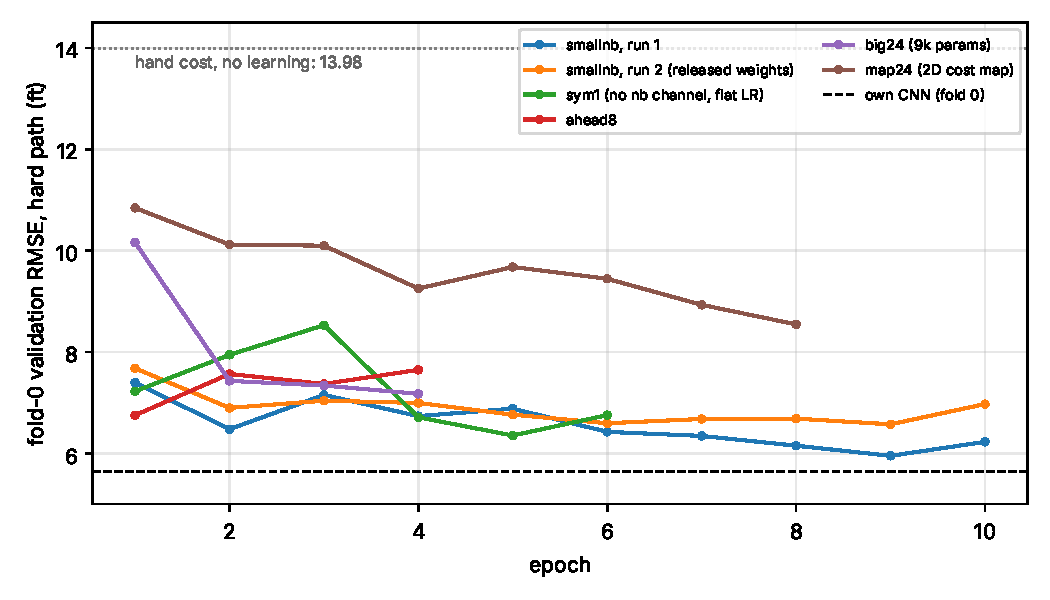
\includegraphics[width=0.75\linewidth]{figures/curves.pdf}
\caption{Fold-0 validation RMSE (hard path) per epoch for all runs. Dashed: our CNN on the same fold.}\label{fig:curves}
\end{figure}

\subsection{Hidden test set}
We submitted the released fold-0 \emph{smallnb} model, trained on 4/5 of the training wells, as a late submission. The test-time neighbour field uses all 773 wells, and the output is the hard path. Table~\ref{tab:lb} compares it with our CNN and with the competition winner.

\begin{table}[h]\centering\small
\begin{tabular}{lrrr}
\toprule
Submission & Params & Private RMSE & Public RMSE\\\midrule
Soft segment-Viterbi, smallnb (this work) & 1{,}271 & 7.724 & 9.551\\
Own CNN, ConvNeXt-small cost volume & ${\sim}$50M & 6.384 & 6.600\\
Competition winner (leaderboard) & -- & 5.639 & --\\
\bottomrule
\end{tabular}
\caption{Kaggle hidden-test scores (late submissions).}\label{tab:lb}
\end{table}

The private-score gap to our CNN (1.34\,ft) is somewhat larger than on fold 0 (0.94\,ft). The public split is smaller, and as Sec.~\ref{sec:err} shows, the model's errors are dominated by a few wells with 20--30\,ft branch errors, to which a small split is very sensitive.

\subsection{Where the error lies}\label{sec:err}
We decode all fold-0 wells with the released weights. Overall hard RMSE is 6.58, with the soft path at 6.97.
\paragraph{Concentration.} The error is concentrated in few wells (Table~\ref{tab:conc}). Without the worst 20 wells the remaining 135 wells score 3.88\,ft.
\begin{table}[h]\centering\small
\begin{tabular}{lrrrrrr}
\toprule
Worst wells removed & 0 & 1 & 3 & 5 & 10 & 20\\\midrule
RMSE of remaining wells (ft) & 6.58 & 6.22 & 5.72 & 5.35 & 4.68 & 3.88\\
Share of squared error removed & -- & 11\% & 26\% & 36\% & 53\% & 70\%\\
\bottomrule
\end{tabular}
\caption{Error concentration on fold 0.}\label{tab:conc}
\end{table}

\paragraph{Growth along the lateral.} RMSE by position decile is 2.3, 4.0, 4.6, 5.5, 6.4, 7.2, 7.7, 8.0, 8.2, 8.7\,ft. Once the path leaves the correct layer it rarely recovers.

\paragraph{Failure mode.} Fig.~\ref{fig:sspace} shows wells in $\Sv$. The grid best fit always tracks the truth. The prediction follows the truth until a single junction, then continues on a different branch:
\begin{itemize}
\item the opposite dip direction (2d35f86d);
\item a shallower dip than the truth (d7eb0be8, which rejoins the truth 3{,}000\,ft later);
\item the wrong direction from the very first decision (53134831).
\end{itemize}
Typical wells (d41beaf2, 3.1\,ft) show only small local deviations. The true paths have far fewer kinks than the predicted ones, which suggests a missing curvature prior. We set no transition penalty in this study.

\paragraph{Near-tied alternatives.} For each well we extract distinct alternative paths: the best path forced through each lattice node (min-marginals), kept only if it is more than 4\,ft RMS away from all paths already chosen. The median extra cost of the 2nd/3rd/4th path is only 0.31/0.52/0.73. Picking the best of the top-$k$ paths with knowledge of the truth (an oracle) gives 5.18 ($k{=}2$), 4.81 ($k{=}3$) and \textbf{4.10}\,ft ($k{=}4$), against 6.58 for the top path.

In many of the worst wells the correct branch is the 3rd or 4th path (Table~\ref{tab:topk}, Fig.~\ref{fig:topk}). In 896d15b9 the soft path is correct (1.4\,ft) while the hard path is not (24.1\,ft): the model was nearly indifferent between two branches. In two wells (53134831, d7eb0be8) none of the top four paths takes the correct branch.

\begin{table}[h]\centering\small
\begin{tabular}{lrrrr}
\toprule
Well & Top path & Best of top 4 (rank) & Extra cost & Soft path\\\midrule
2d35f86d & 18.4 & 1.3 (4) & 0.32 & 18.6\\
896d15b9 & 24.1 & 3.0 (4) & 0.33 & 1.4\\
fb73b13a & 17.0 & 3.8 (3) & 0.30 & 17.3\\
9def2eb2 & 20.2 & 5.6 (4) & 0.33 & 13.9\\
c03fba65 & 14.3 & 2.7 (3) & 0.24 & 3.6\\
53134831 & 26.6 & 21.3 (2) & 0.17 & 27.3\\
d7eb0be8 & 17.3 & 17.3 (1) & -- & 17.9\\
\bottomrule
\end{tabular}
\caption{RMSE (ft) of the top Viterbi path, the best of the top-4 distinct paths, and the soft path on high-error wells.}\label{tab:topk}
\end{table}

\begin{figure}[p]\centering
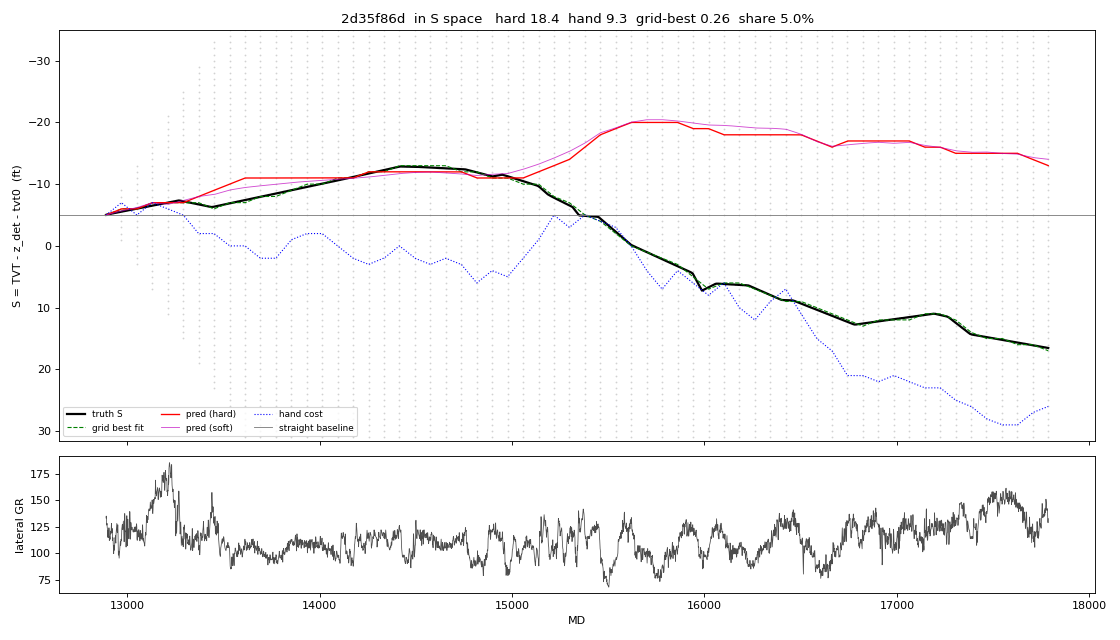
\includegraphics[width=0.95\linewidth,height=0.27\textheight,keepaspectratio]{figures/S_2d35f86d.png}\\[2pt]
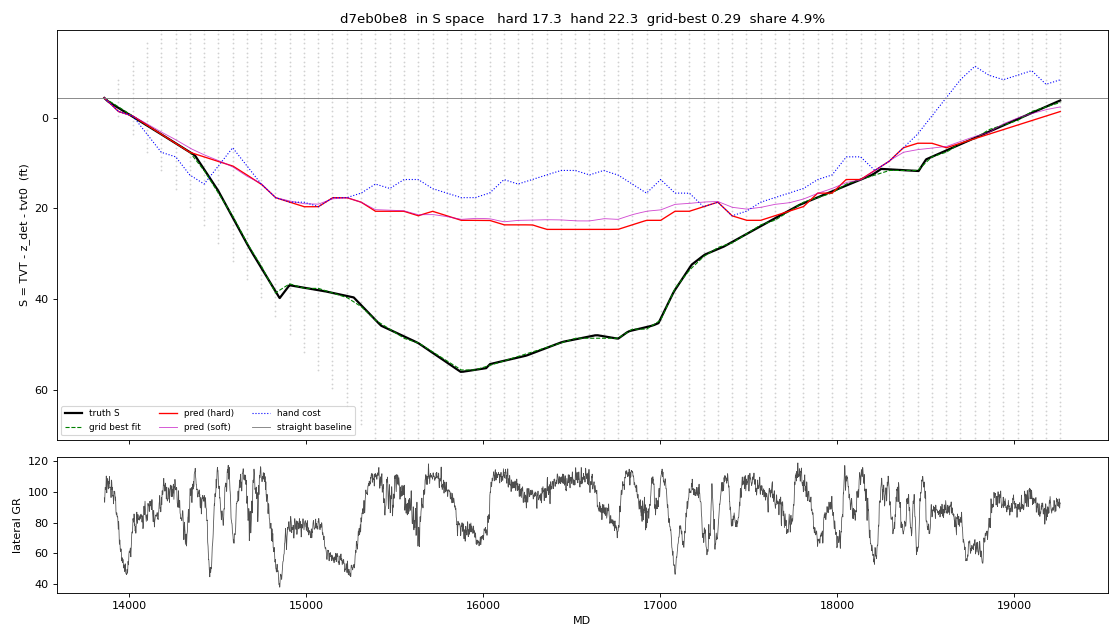
\includegraphics[width=0.95\linewidth,height=0.27\textheight,keepaspectratio]{figures/S_d7eb0be8.png}\\[2pt]
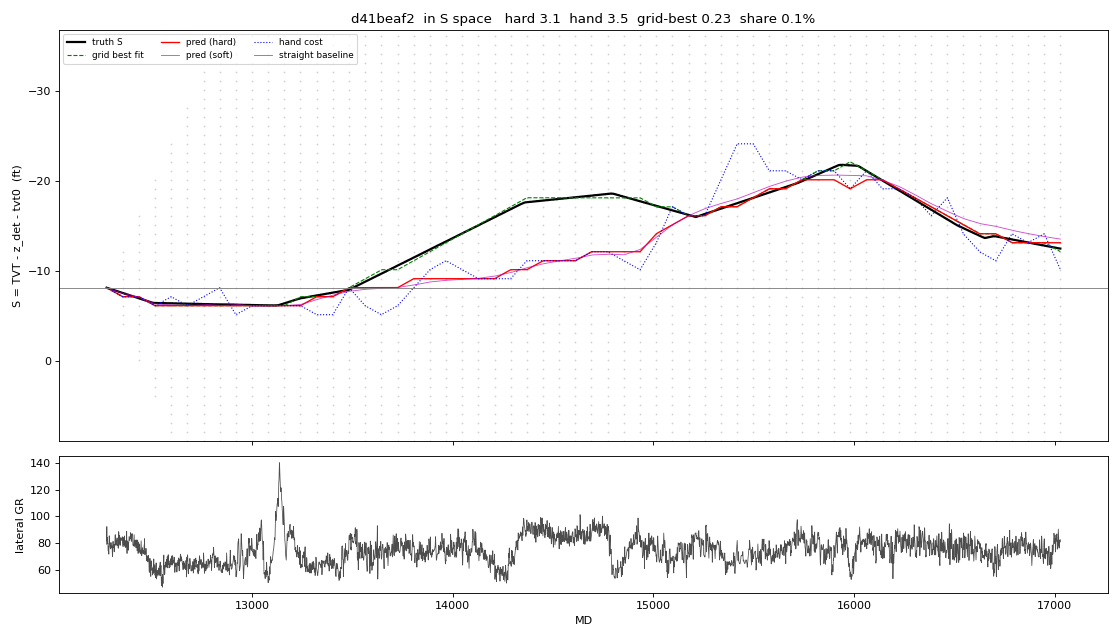
\includegraphics[width=0.95\linewidth,height=0.27\textheight,keepaspectratio]{figures/S_d41beaf2.png}
\caption{Predictions in the structural coordinate $\Sv$ (larger $\Sv$ plotted downwards) for two high-error wells and one typical well, with the lateral GR below each panel. Black: truth; dashed green: grid best fit; red: hard path; magenta: soft path; blue dotted: hand-cost Viterbi; grey: straight baseline; grey dots: anchors.}\label{fig:sspace}
\end{figure}

\begin{figure}[p]\centering
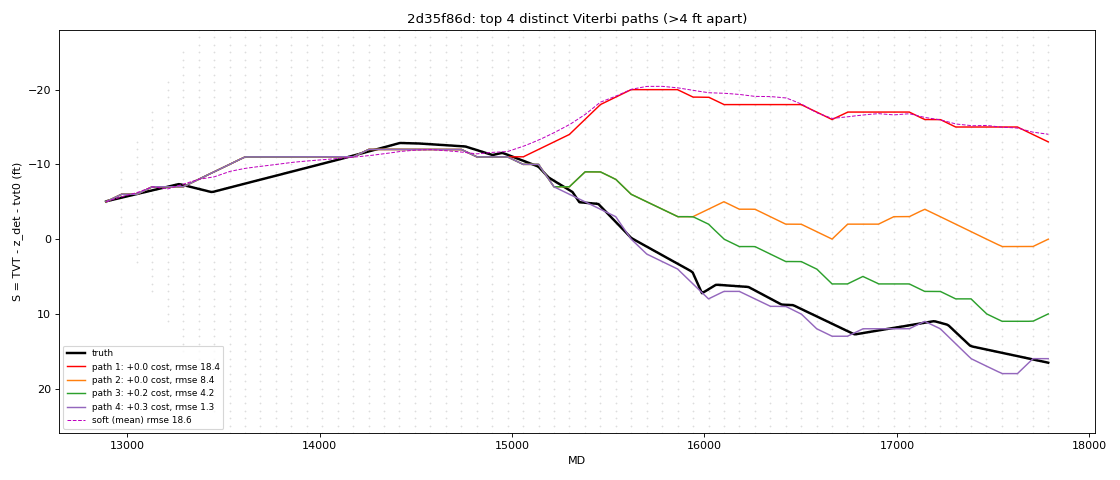
\includegraphics[width=0.95\linewidth,height=0.27\textheight,keepaspectratio]{figures/K_2d35f86d.png}\\[2pt]
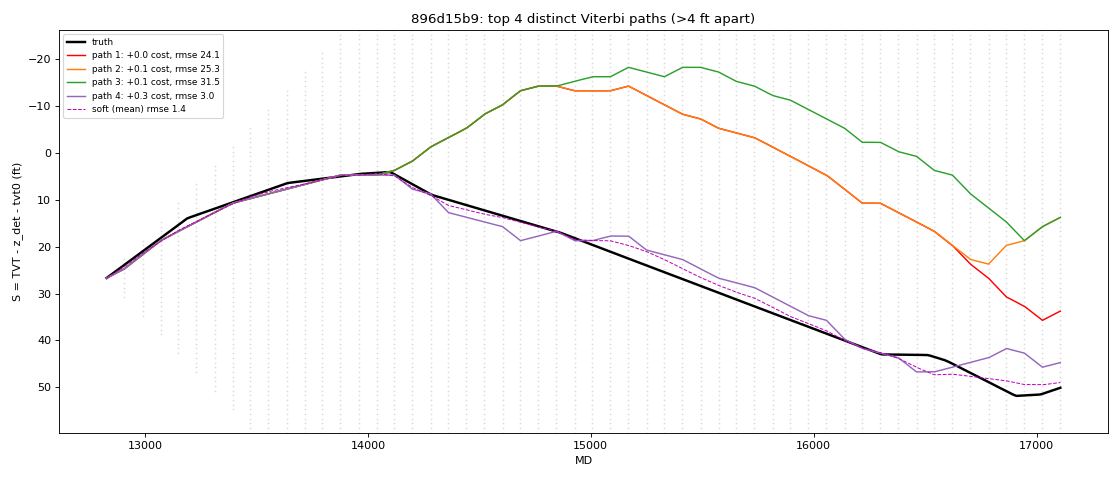
\includegraphics[width=0.95\linewidth,height=0.27\textheight,keepaspectratio]{figures/K_896d15b9.png}\\[2pt]
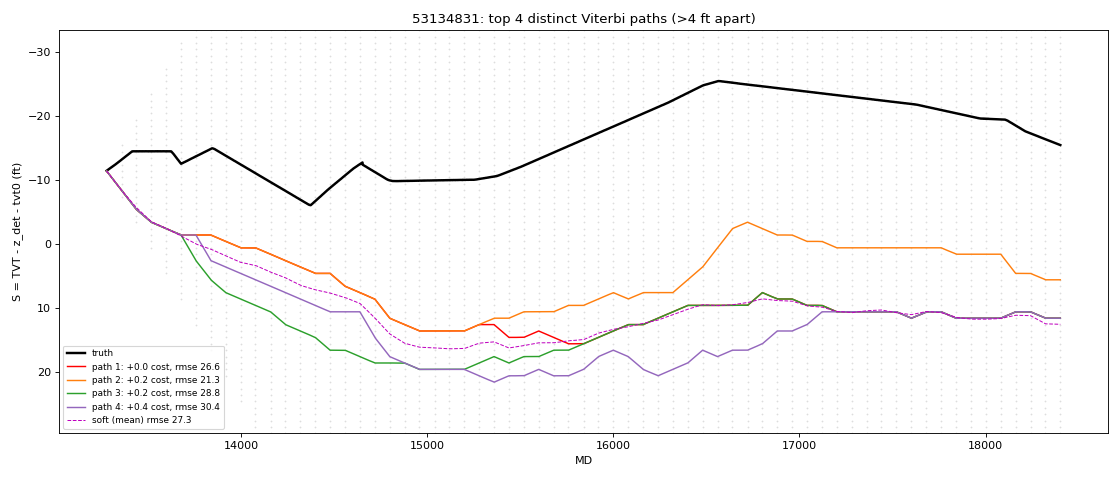
\includegraphics[width=0.95\linewidth,height=0.27\textheight,keepaspectratio]{figures/K_53134831.png}
\caption{Top-4 distinct Viterbi paths of the trained cost network, with their extra cost relative to the best path and their RMSE. In the first two wells a path within 0.3 cost units of the optimum is correct to 1--3\,ft; in the third, no candidate takes the correct (upward) branch.}\label{fig:topk}
\end{figure}

\section{Discussion}
\paragraph{Soft versus hard path.} Training minimises the MSE of the \emph{expected} path. Under ambiguity this rewards placing the anchors between branches, which for an RMSE metric is the Bayes-optimal response if the branch probabilities are calibrated. In practice the learned temperature becomes small ($T\approx0.05$), so the soft and hard paths usually coincide. The released model performs better with the hard path (6.58 vs 6.97); 896d15b9 is the notable exception.

\paragraph{What limits the model.} Neither lattice resolution (0.25\,ft) nor a lack of candidate paths explains the error: a correct or nearly correct branch is usually within a small cost margin. The local, chunk-wise cost cannot separate branches whose GR signatures are similar over 240\,ft windows. This points to three directions:
\begin{enumerate}
\item scoring complete candidate paths with whole-lateral evidence (full-path GR correlation, number of kinks, agreement with the neighbour field), i.e.\ a second-stage re-ranker over the top-$k$ paths;
\item a learned curvature (slope-change) term in the segment transition, matching the observed piecewise-linear geology;
\item a loss that also penalises the hard path or anneals $T$, so that training widens the margin between the true branch and its competitors.
\end{enumerate}

\paragraph{Model size.} With about $4\times10^4$ times fewer parameters, the cost network trained through the DP is 0.3--0.9\,ft behind a large CNN on the validation fold. The structural model supplies the prior (straight segments, dip limit, global consistency), and the network only has to rank local candidates.

\paragraph{Limitations.} All validation results are on a single fold. Runs of the same configuration differ by ${\approx}0.6$\,ft. The test submission uses a single fold model trained on 80\% of the wells. Training was CPU-bound, which prevented multi-seed or 5-fold evaluation and full training of the larger cost networks.

\section{Reproducibility}
The accompanying folder contains the code (\texttt{code/}), the configurations of every run in Table~\ref{tab:abl} (\texttt{code/README.md}) and the released weights (\texttt{weights/vs\_smallnb\_best.pt}: 1{,}271 parameters, fold-0 model, best epoch; learned $w=0.877$, $T=0.049$). Fold-0 evaluation, error analysis, top-$k$ paths and test prediction run from the released weights without retraining.

{\small
\bibliographystyle{plainnat}
\bibliography{refs}}
\end{document}
